%% Copernicus Publications Manuscript Preparation Template for LaTeX Submissions
%% ---------------------------------
%% This template should be used for copernicus.cls
%% The class file and some style files are bundled in the Copernicus Latex Package, which can be downloaded from the different journal webpages.
%% For further assistance please contact Copernicus Publications at: production@copernicus.org
%% https://publications.copernicus.org/for_authors/manuscript_preparation.html


%% Please use the following documentclass and journal abbreviations for discussion papers and final revised papers.


%% 2-column papers and discussion papers
%\documentclass[acp, manuscript]{copernicus}
\documentclass[acp]{copernicus} % final format

%% \usepackage commands included in the copernicus.cls:
%\usepackage[german, english]{babel}
%\usepackage{tabularx}
%\usepackage{cancel}
%\usepackage{multirow}
%\usepackage{supertabular}
%\usepackage{algorithmic}
%\usepackage{algorithm}
%\usepackage{amsthm}
%\usepackage{float}
%\usepackage{subfig}
%\usepackage{rotating}


\begin{document}

\title{Brewer Spectrophotometer laboratory wavelength characterization with a tunable-laser implications to the Brewer ozone retrieval}


% \Author[affil]{given_name}{surname}
\Author[1,2]{Alberto}{Redondas}
\Author[3]{Saulius}{Nevas}
\Author[4,2]{Alberto} {Berjón}
\Author[3]{Meelis-Mait} {Sildoja}
\Author[1,2]{Sergio F.}{León-Luis}
%\author[6]{Omar el Gawhary} 
%\author[7]{Ilias Fountoulakis}


\affil[1]{Agencia Estatal de Meteorología, Izaña Atmospheric Research Center, Spain}
\affil[2]{Regional Brewer Calibration Center for Europe, Izaña Atmospheric Research Center, Tenerife, Spain}
\affil[3]{Physikalisch-Technische Bundesanstalt (PTB), Braunschweig and Berlin, Germany}
\affil[4]{University of La Laguna, Department of Industrial Engineering, S.C. de Tenerife, Spain}





\runningtitle{Brewer Wavelength Calibration}

\runningauthor{Redondas}

\correspondence{Alberto Redondas (aredondasm@aemet.es)}



\received{}
\pubdiscuss{} %% only important for two-stage journals
\revised{}
\accepted{}
\published{}

%% These dates will be inserted by Copernicus Publications during the typesetting process.


\firstpage{1}

\maketitle



\begin{abstract}

In this work we present the wavelength calibration of the traveling reference Brewer of the RBCC-E  \url{http://rbcce.aemet.es}  at PTB in Braunschweig, Germany. The wavelength calibration is needed for calculation of the ozone absorption coefficient used by the Brewer ozone algorithm. In order to validate the standard procedure for determining Brewer’s wavelength calibration an  experiment using an tunable laser light source have been performed within the ATMOZ project. In this experiment we compare the standard procedure of wavelength calibration performed to Brewer instrument uses to the calibration results obtained using the PTB laser facility. This allows to check the methodology measuring directly the ozone absorption coefficient without the assumptions made by the operational methodology.  The results of the laser experiment reproduces the  the operational methodology used and shows that there is a underestimation of 0.8\%  due the use of the parametrized slit function. 
\end{abstract}

\copyrightstatement{TEXT}

\section{Background}

The wavelength calibration is needed for calculation of the ozone absorption coefficient used by the Brewer ozone algorithm. The usual wavelength calibration procedure is performed by analyzing recorded emission lines of the spectral discharge lamps  usually Mercury (Hg), Cadmium (Cd) , and Zinc (Zn) detailed on Table \ref{tab:dsp_lines}, determining their central wavelengths and the corresponding FWHM (full width half maximun)   and the relation between the positions of the grating  and the  corresponding wavelengths  (dispersion relation) for the operational wavelengths used for the ozone determination. The Brewer spectrophotometer have two operating  modes. The ozone one, used for ozone measurement, is performed with the diffraction grating at a fixed position while  the six operational wavelengths are measured by  rotating slit mask.  The scanning mode, used for the spectral UV measurements, is performed while the slits are fixed and the spectral scan is carried out by turning the diffraction grating. To obtain the ozone absorption coefficient the instrumental slit function is convoluted whit the Bass \& Paur ozone cross section.
The use of the of the laser tunable source allow us to:
\begin{itemize}

    \item Calculate the ozone absorption coefficient directly.  The ozone absorption coefficient  determination  uses the scan the spectral lines so that dispersion relation is used to convert grating position in micrometer steps to wavelengths assuming a quadratic relation. Scanning with the laser around the ozone operational wavelengths we can determine the instrumental slit functions directly and weight them with the ozone cross sections without need for the assumptions of the slit functions and the dispersion relations used in the normal operational procedure.
    \item Calculate the dispersion relation based on regularly spaced reference spectral lines provided by the tunable laser instead of the irregularly distributed  emission lines of the  Hg, Cd and Zn spectral lamps. 
\end{itemize}

%The objective of this work is  to validate the standard procedure for the brewer spectrophotometer, For that we compare  to do that we perform 3 experiments, the standard procedure described on secion 2, the experiments results obtained with the laser , using the brewer on ozone mode (the lases scans ) and finally using the laser

During the experiment we perform three measurements: 
\begin{enumerate}


\item The standard method of the dispersion measurements using spectral lamps described on secion 2.

\item  Direct dispersion measurements (Laser scanning). 
While Brewer is measuring in ozone mode and in aerosol mode, the laser will scan around (±2\unit{nm}) the six Brewer slits with a step of 0.05\unit{nm} for different grating positions 

%(ozone and aerosol). 


\item  Dispersion measurements using tunable laser (Brewer scanning) : While Laser is emitting in a fixed wavelength, the Brewer will scan around  this wavelength (±2\unit{nm}) moving the grating and using the 6 slits. This process will be repeated 16 times, using wavelengths ranging from 290 \unit{nm} to 365 $\unit{nm}$ with an increment of 5$\unit{nm}$.  This allow us to estimate the error due to the lack of spectral lines on the end wavelength range of the brewer spectrometer and the fact that that the emission lines are not equally spaced.

%\item 
\end{enumerate}







\section{The Brewer spectrometer calibration}
\label{sec:calibration}


The Brewer instrument measures the intensity of direct sunlight at six wavelengths ($\lambda$) in the UV (303.2, 306.3, 310.1, 313.5, 316.8, and 320.1~\unit{nm}) each covering a bandwidth of 0.5~\unit{nm} (resolution power $\lambda/\delta\lambda$ of around 600). The spectral measurement is achieved by a holographic grating in combination with a slit mask which selects the channel to be analyzed by a photomultiplier. The longest four wavelengths are used for the ozone calculation. Based on the Lambert-Beer law, the total ozone column in the Brewer algorithm can be expressed as:

\begin{equation}
	\label{eq:ozone}
	X = \frac{{F - ETC }}{\alpha  \mu }\
\end{equation}

where $F$ are the measured double ratios corrected for Rayleigh effects, $\alpha$ is the ozone absorption coefficient, $\mu$ is the ozone air mass factor, and $ETC$ is the extra-terrestrial constant. The $F$, $\alpha$ and $ETC$ parameters are weighted functions at the operational wavelengths with weighting coefficients $w$:
      
\begin{equation}	
	F = \sum\limits_i^4 {{w_i} {F_i} - \frac{p} {p_0} \beta_i \mu }
\end{equation}
      
\begin{equation}	
	\alpha = \sum\limits_i^4 {{w_i} {\alpha_i} }
\end{equation}

\begin{equation}	
	ETC = \sum\limits_i^4 {{w_i} {{F_0}_i} }
\end{equation}

where, $\beta_i$ are the Rayleigh coefficients,  $p$ is the climatological pressure at the measurement site, $p_0$ is the pressure at sea level, and $F_0$ are the individual extra-terrestrial constants at each wavelength. The weights $w=[1,-0.5,-2.2, 1.7]$ have been chosen so as to minimize the influence of SO$_2$ and verify:
      
\begin{equation}	
	\sum\limits_i^4 {{w_i} }=0
\end{equation}
     
\begin{equation}	
	\sum\limits_i^4 {{w_i} {{\lambda}_i} }=0
\end{equation}

This widely eliminates absorption features which depend, in local approximation, linearly on the wavelength, like for example the contribution from aerosols.

We can divide the calibration in three steps:

\begin{enumerate}
	\item Instrumental, wavelength, and ETC transfer: the Instrumental calibration includes all the parameters that affect the measured counts ($F$), in particular Dead Time correction, Temperature coefficients and  Filter attenuation.
	\item Wavelength calibration to determine the ozone absorption coefficient: the so-called ``dispersion test'' are used to obtain the particular wavelength for the instrument and the slit, or instrumental function, of each spectrophotometer. Note that the precise wavelengths of every Brewer spectrophotometer are slightly different from instrument to instrument. 
	\item Finally, the ETC transfer is performed by comparison with the reference or, in the case of the reference instruments, by the Langley method.
\end{enumerate}

%The calibration process can be considered as cycle changes. Instrumental and/or wavelength calibration will affect the final ETC and changes in the wavelength calibration will affect also to the final ETC. 

The Brewer wavelength calibration follows the operative procedure \citep{Grobner1998, kerr2002new} used by the Regional Brewer Calibration Center-Europe (RBCC-E) at the calibration campaigns. In summary the individual wavelengths in the Brewer measurement set are located at the focal plane of the spectrometer through the use of a stainless steel mask of seven slits, the particular wavelength is determined by analyzing the measurements of  a series of discharge lamps on a process so-caled dispersion-test wich determines the central wavelength and Full Width Half Maximum (FWHM) of every slits. Then the  wavelength setting is optimized to minimize the effect of wavelength shift during the operation of the instrument by the sun-scan test \citep{sun_scan_ios}. And finally the ozone absorption coefficient is determined.   


The  ozone absorption coefficient is defined as:

\begin{equation}
\widetilde \alpha (X,\mu ) = \sum {{w_i}} \frac{{\int {\alpha (\lambda )*S(\lambda ,\lambda ')*} F(\lambda ,\lambda ',X,\mu )d\lambda '}}{{\int_{}^{} {S(\lambda ,\lambda ')*F(\lambda ,\lambda ',X,\mu )d\lambda '} }}
\end{equation}

Where $S$ is the instrument slit function for the corresponding wavelength  $F$is the sun spectra mostly which depends on the UV. range of the ozone concentration and airmass, and $\sigma$ the ozone cross section at  temperature, $-$46.3\, \unit{\degree C} for Dobson Network
and $-$45\, \unit{\degree C} for Brewer instruments. 

The Brewer operative method, perform the following assumptions.
\begin{enumerate}
	\item Use  “ideal” slits,  the slits function are parametrized as a trapezoid; and isosceles triangle truncated at 0.82 height.
	\item Stray light is not considered the transmission is outside the triangle. 
	\item The FWHM of the triangle is dependent of the slit as is derived from the dispersion test.
	\item The ozone cross section  is Bass \& Paur absorption coefficient.
 	\item Solar Spectra is not considered ,  ($F$==1)
\end{enumerate}

With this assumption the ozone effective absorption is essentially the same as the approximation method of \citet{Bernhard2005}  used on Dobson Spectrometer. (see Eq.~\ref{eq:conv}).


      \begin{equation}
      \label{eq:conv}
            %\alpha_i = {{\int {\sigma(\lambda)\, {S_i}(\lambda)\, \text{d}\lambda } }
            %\over{\int_{}^{} {{S_i}(\lambda )\text{d}\lambda } }}
            \alpha_i = \frac{\int \sigma(\lambda) S_i(\lambda) \mbox{d}\lambda}{\int S_i(\lambda) \mbox{d}\lambda}
      \end{equation}


\subsection{Dispersion Test}

The Brewer spectrophotometer is constructed with either one or two modified Ebert–Fastie type monochromators single or double Brewer. The first monochromator disperses the incoming radiation onto six exit slits. In the case of the double Brewer , the six exit slits  (intermediate slits) of the first monochromator are the entrance slits to a second monochromator that is used in the recombining mode. The wavelength is be selected by choosing one of the six exit slit (ozone mode) or rotating the grating (uv mode). The rotation of the grating is managed by a micrometer.The drive mechanism, consisting of a motor-driven micrometer linked to an arm that rotates the grating. The smallest wavelength increment one motor step varies steadily from approximately 8.0 pm to 7.0 pm ( 0.0080 \unit{nm} ). 

The dispersion relation (which gives the  relation between the micrometer step and wavelength ) is determined scanning the emission lines. The brewer scan every 10 steps (~0.6A), the central step and the FWHM are calculated assuming a isosceles triangle. The both sides of the peak are  fitted to straight line  ,taking only the observations above 20\%  and bellow 80\% of the normalized peak, the central point is calculated by the intersection point and the FWHM is the with of the triangle. (Figure x). Then the dispersion relation is calculated as quadratic polynomial or using the cubic approximation \citep{Grobner1998}. This relation is used to transform the previously determined central and FWHM in micromenter steps to wavelength scale.


% mercury test
   The Stability of the wavelength calibration during the brewer operation  is checked by the measure of the internal HG line,in most of the brewer a 302 \unit{nm} double line is used, (302.150 nm and 302.347 nm) due the its proximity to the operational wavelengths however on brewer \#185 and in increased number of brewer the test is  performed using the more powerfull 296.7 \unit{nm} line. The test taking 12 measurements, 10 steps of the micrometer motor apart, of the intensity from the mercury lamp on slit 0. The registered peak is compared to a reference stored one. The comparsion the scans is done by shifting the two scans against each other and calculating the correlation coefficient between the two after each shift. The interpolated step number resulting in the maximum of the correlation is the reference micrometer position.(\citep{savastiouk2005improvements} ).If the required adjustment of the micrometer position is more than one and a half steps,  the test is repeated.Due the hg test the accuracy of the wavelength setting cannot be better than about micrometer step (0.86) which, determined by is limited by one and half step correction, this translates in ozone abortion coefficient change approximately of 0.10 \unit{atm $cm^-1$}  which gives approximately a  0.3\% in ozone concentration.
   % the error of a step funciotn of  1.5 step wide =   1.5 / sqrt(3)  is 0.86
  


\subsection{Sun Scan}
\citet{savastiouk2005improvements} 


\section{ OPO experiment}

\subsection{Laser Instrumental Setup}

The facility PLACOS (Pulsed Laser for Advanced Characterisation of Spectroradiometers) at Physikalisch-Technische Bundesanstalt (PTB). This system is employed for the spectral characterisation of array spectroradiometers throughout the spectral range from 220 \unit{nm} to 2200 \unit{nm}. It uses an optical parametric oscillator (OPO) and a second-harmonic generator (SHG). The pump radiation for the OPO crystals is delivered by the 3rd harmonic of a Nd:YAG laser (355 \unit{nm}). The resulting signal of the OPO covers the spectral range from approximately 410 \unit{nm} up to 2200 \unit{nm}. The SHG unit enables an extended range down to 220 \unit{nm}.  (Figure \ref{fig:opo})


% monitor description
% accuracy


In contrast with the standard procedure where the Brewer scans the spectral lamps lines, on this experiment the brewer measure in ozone mode, the grating is fixed on the ozone position and measure the laser system with the seven slits. The opo scan every 0.01 \unit{nm}  This experiment  measure the seven slits (the slit  \#1 is blocked) were the OPO system . The experiment is complemented using the laser as source of spectral lines covering the range from 290\unit{nm} to 360 \unit{nm} in regular steps of 5 \unit{nm}, the brewer resolution of the scan is doubled on the experiment and is done every 5 \unit{nm}.



\subsubsection{PMT No linearity}

The brewer photomultiplier (PMT) is not linear with pulsed sources, the PMT manual advised  we must change PMT electronics configuration for pulsed sources.   As the main objective is to validate the operational wavelength calibration of the brewer  we decide to maintain the instrument configuration as operated in field and correct the no-linearity using the simultaneous measures of the laser intensity.


The ratios between the measured counts of the  brewer to the recorded laser measurements are shown on figure  \ref{fig:no}. The no linearity is evident with regions with hysteresis, near $10^4$  Brewer counts/seconds ,  regions were the correction is not reliable  around $10^3$ and  with counts lower than 100. As we can control the intensity of the laser, we are able to work on the “flats regions” and apply the determined the nolinear correction. This correction will not affect to the calculation of the central wavelength but affect the determination of FWHM (Figure \ref{fig:slitcor}) if not correction is applied.

One of the limitations of this correction is to work with low signals, the correction is not reliable for counts lower than 100. Also we observe (Figure \ref{fig:laser_log}) as the recorder dark counts (measurements performed with the blocked slit nº1), were highest immediately after exposing the PMT to the laser light. The dark signal was then gradually decreasing with time. The dark values of the PMT may show a fast decay after the excitation, which may cause the values for slit \#1 (measured immediately after slit \#0) be higher than for some other slits, measured later.

\subsubsection{Slit parametrization }

The brewer algorithms assume a trapezoidal slit, cut a 0.87 of the height (Figure \ref{fig:param}), with the  center and fwhm  calculated for every slit by the dispersion. This experiment allow us to estimate the difference on the ozone calculation if we use the measured slit instead of the parametrised one. We calculate the ozone absorption coefficient for the four ozone cross section evaluated in the  "ACSO" comitee ("Absorption Cross Sections of Ozone") ( \citet{orphal2016absorption}.

Two of this are versions of  Bass and Paur~(1985) cross-sections denoted as Brewer operational (Brw), IGACO quadratic coefficient (B\&P), the xs of  Daumont Brion Malicet (DBM) (\citet{ daumont_ozone_1992}, \citet{brion_high-resolution_1993}, and \citet{malicet_ozone_1995} ) , and 
 the newly recommended data set for ozone ground based calculation  Serdyuchenco, Groshelev, Weber (SGW) \citep{serdyuchenko_high_2012,gorshelev_high_2012,amt-9-4459-2016}. 


Using the measured slit  ,  the effective ozone cross section calculated is $~0.9\%$ higher respect the parametrized brewer slit on the standard procedure (Table \ref{tab:slit_param}) independelty of the cross section used.


\section{Comparison }

The experiment allow us to validate the Brewer standard methodology to perform the wavelength calibration. Using as a reference the direct calculation we compare the operative method using the spectral lamps and using the laser in regular intervals in both methods using the quadratic fit and the cubic fit.

The figure \ref{fig:cw_comp} shows the difference on the central wavelength calculation the quadratic methods shows discrepancies bigger than 0.1 A for wavelength adobe 320 \unit{nm} and much bigger near 350 nm. This is  also indicated by the residuals of the fit quadratic systematic and much bigger than the cubic method (not shown) that shows  the quadratic method is only valid on the ozone range (310-320 nm). The comparison of the FWHM calculation (Figure \ref{fig:cw_comp} ) show a different pattern with a 0.1A difference on the ozone range and with less difference between quadratic and cubic methods.  

The results of the difference to the direct calculation of the ozone absorption coefficient are summarized on the table x, for the six \ref{tab:o3abs_sum}




\conclusions{}

\begin{enumerate}

%\item 
 %We don't find significant differences when different input optics is used for the wavelength characterization, placing the spectral source on the global port, direct port or using the Hg internal lamp are interchangeable for this purposes.

    \item Using the measured slit instead of the paramterized slit increase the ozone absorption coefficient and consequently the calculated ozone in 0.8\%.

    \item The quadratic fit used on the standard algorithm is not suitable outside the ozone range 310-320 nm and shows systematic residuals this is particularly important on the higher range%-> effect o the ozone<-

    \item The comparison of three experiments shows a  maximum difference of 0.3\% if the cubic fit is used, the error in the ozone using direct measurement in ozone mode and operative discharge lamp method is only of 0.1\%. This confirms the standard procedure using on the RBCC-E calibrations.

\end{enumerate}




%% ONE-COLUMN FIGURES

%%f
\begin{figure}[t]
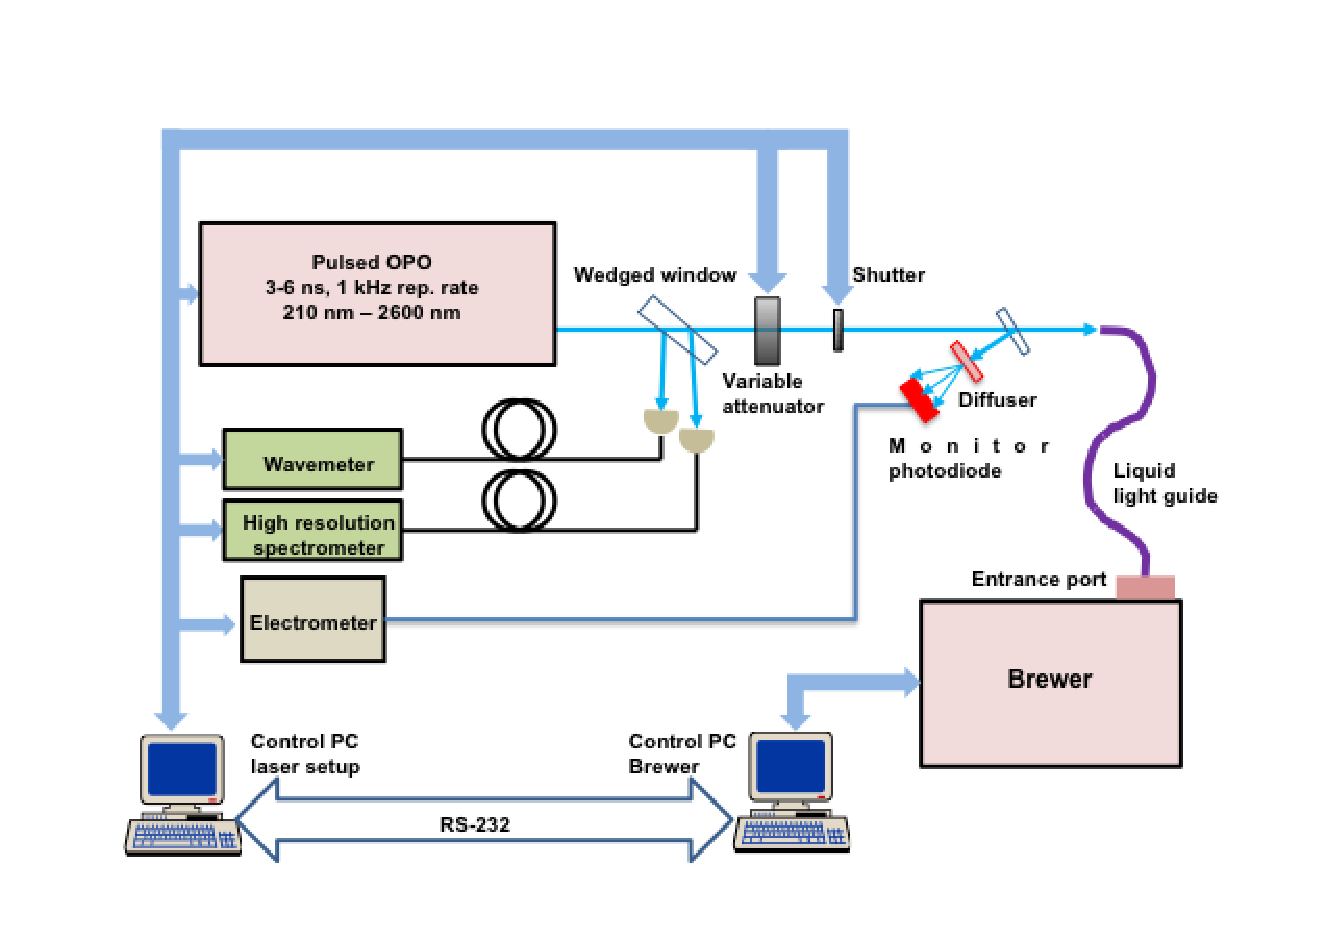
\includegraphics[width=8.3cm]{figures/opo.eps}
\caption{TEXT}
\label{fig:opo}
\end{figure}





%%f
\begin{figure}[t]
\includegraphics[width=8.3cm]{figures/General_NoLinearity_corr.eps}
\caption{ Log-log plot of the normalized ratio of Brewer registered counts to the Laser counts against the brewer counts, the black points shows the experimentally points and the red curve the fit used to correct the brewer measurements.}
\label{fig:no}
\end{figure}

%%f
\begin{figure}[t]
\includegraphics[width=8.3cm]{figures/General_Corrected_vs_uncorrected.png}
\caption{Measurement of the 310 slit (Slit \#4) uncorrected counts per second (black) and no linearly corrected counts, the central wavelength determination is no affected but FWHM is bigger if the correction is not applied, the hysteresis is evident on the asymmetry of the low intensity of the plot, as the method use only the observations between 0.2 and 0.8 of the normalized intensity do not have effect on the calculations.  }
\label{fig:slitcor}
\end{figure}

%


%
\begin{figure}[t]
\includegraphics[width=8.3cm]{figures/General_Laser_Brewer_ozone_mode.eps}
\caption{ Plot of the parametrized slits and the measured slits (dots)  and the different ozone cross sections (left axis) used on effective ozone absorption coefficient brewer ozone calculation.}
\label{fig:param}
\end{figure}


%
\begin{figure}[t]
\includegraphics[width=8.3cm]{figures/General_laser_log.eps}
\caption{ Measurement of the Brewer in ozone mode while the Laser is scanning every 0.1 nm , in blue the measurements of the slit 1 correspond with the dark count.}
\label{fig:laser_log}
\end{figure}

%
\begin{figure}[t]
\includegraphics[width=8.3cm]{figures/General_Laser_scan_dsp.eps}
\caption{ Measurement of the Brewer in ozone mode while the Laser is scanning every 0.1 nm , in blue the measurements of the slit 1 correspond with the dark count.}
\label{fig:laser_dsp}
\end{figure}

\begin{figure}[t]
\includegraphics[width=8.3cm]{figures/General_central_comparison.eps}
\caption{ Central Wavelength determination differences between the direct determination and the scanning methods: with the laser in equally spaced lines every 5nm and the discharge lamps using in both cases quadratic and cubic fitting}
\label{fig:cw_comp}
\end{figure}

\begin{figure}[t]
\includegraphics[width=8.3cm]{figures/General_fwhm_comparison.eps}
\caption{ FWHM determination differences between the direct determination and the scanning methods: with the laser in equally spaced lines every 5nm and the discharge lamps using in both cases quadratic and cubic fitting}
\label{fig:fwhm_comp}
\end{figure}

\begin{figure}[t]
\includegraphics[width=8.3cm]{figures/General_DSP_QUAD_RES.eps}
\caption{ Residual of the quadratic fit}
\label{fig:dsp_residual_quad}
\end{figure}


\begin{figure}[t]
\includegraphics[width=8.3cm]{figures/General_brewer_scan_cubic_residual.eps}
\caption{ Residual of the cubic fit}
\label{fig:dsp_residual_cubic}
\end{figure}

%\subsection{HEADING}
%TEXT
%\subsubsection{HEADING}
%TEXT


%\conclusions  %% \conclusions[modified heading if necessary]
%TEXT

%% The following commands are for the statements about the availability of data sets and/or software code corresponding to the manuscript.
%% It is strongly recommended to make use of these sections in case data sets and/or software code have been part of your research the article is based on.

\codeavailability{TEXT} %% use this section when having only software code available


\dataavailability{TEXT} %% use this section when having only data sets available


\codedataavailability{TEXT} %% use this section when having data sets and software code available


%\clearpage

\begin{table}[t]
\caption{Emission lines of the Discharge Lamps used for Brewer calibration}
\begin{tabular}{lll}
\tophline
Lamp           & Line (nm) & Slits \\
\middlehline
Mercury (Hg)   & 289.36    & 0–1   \\
Hg             & 296.728   & 0–3   \\
Zinc (Zn)      & 301.836   & 0–5   \\
Zn             & 303.578   & 0–5   \\
Cd (multiplet) & 308.082   & 0-5   \\
Cd             & 313.3167  & 0–5   \\
Cd             & 326.1055  & 0–5   \\
Zn             & 328.233   & 0–5   \\
Hg             & 334.148   & 0–5   \\
Cd             & 340.3652  & 0–5   \\
Cd             & 349.995   & 4–5   \\
Cd (multiplet) & 361.163   & 5     \\
\bottomhline
\end{tabular}
\belowtable{} % Table Footnotes
\label{tab:dsp_lines}
\end{table}


%\clearpage

\begin{table}[t]
\caption{Ozone Absorption Coefficient in atm $cm^-1$ calculated using  four absorption cross sections, }
\begin{tabular}{lll}
\tophline
     & Parametrized & Measured \\
\middlehline
BRW  & 0.3381       & 0.3407   \\
B\&P & 0.3330       & 0.3360    \\
DMB  & 0.3483       & 0.3514   \\
SDK  & 0.3392       & 0.3422    \\
\bottomhline
\end{tabular}
\belowtable{} % Table Footnotes
\label{tab:slit_param}
\end{table}


\begin{table*}[t]
\caption{Ozone Absorption Coefficient in atm $cm^-1$ calculated using  four absorption cross sections, }
\begin{tabular}{lllllll}
\tophline
     & brw\_scan & ptb\_scan & opo\_quad & opo\_cubic & lamp\_quad & lamp\_cubic \\
\middlehline
SGW   & 0.3409    & 0.3368    & 0.3442    & 0.342      & 0.3446     & 0.3412      \\
ratio & 1         & 0.9881    & 1.0096    & 1.0033     & 1.0108     & 1.001      
\bottomhline
\end{tabular}
\belowtable{} % Table Footnotes
\label{tab:o3abs_sum}
\end{table*}

%\appendix
%\section{}    %% Appendix A
%\subsection{}     %% Appendix A1, A2, etc.
%\noappendix       %% use this to mark the end of the appendix section

%% Regarding figures and tables in appendices, the following two options are possible depending on your general handling of figures and tables in the manuscript environment:

%% Option 1: If you sorted all figures and tables into the sections of the text, please also sort the appendix figures and appendix tables into the respective appendix sections.
%% They will be correctly named automatically.

%% Option 2: If you put all figures after the reference list, please insert appendix tables and figures after the normal tables and figures.
%% To rename them correctly to A1, A2, etc., please add the following commands in front of them:

%\appendixfigures  %% needs to be added in front of appendix figures

%\appendixtables   %% needs to be added in front of appendix tables




%% Please add \clearpage between each table and/or figure. Further guidelines on figures and tables can be found below.



%\authorcontribution{TEXT} %% optional section
%\competinginterests{TEXT} %% this section is mandatory even if you declare that no competing interests are present
%\disclaimer{TEXT} %% optional section

\begin{acknowledgements}
This work has been supported by the European Metrology Research Programme (EMRP) within the joint research project ENV59 “Traceability for atmospheric total column ozone” (ATMOZ).  The  EMRP  is jointly funded by the EMRP participating countries within EURAMET and the European Union. 

\end{acknowledgements}




%% REFERENCES

%% The reference list is compiled as follows:

%\begin{thebibliography}{}
%\bibitem[AUTHOR(YEAR)]{LABEL}
%REFERENCE 1
%\bibitem[AUTHOR(YEAR)]{LABEL}
%REFERENCE 2
%\end{thebibliography}

%% Since the Copernicus LaTeX package includes the BibTeX style file copernicus.bst,
%% authors experienced with BibTeX only have to include the following two lines:

 \bibliographystyle{copernicus}
 \bibliography{wv_brewer.bib}
%%
%% URLs and DOIs can be entered in your BibTeX file as:
%%
%% URL = {http://www.xyz.org/~jones/idx_g.htm}
%% DOI = {10.5194/xyz}


%% LITERATURE CITATIONS
%%
%% command                        & example result
%% \citet{jones90}|               & Jones et al. (1990)
%% \citep{jones90}|               & (Jones et al., 1990)
%% \citep{jones90,jones93}|       & (Jones et al., 1990, 1993)
%% \citep[p.~32]{jones90}|        & (Jones et al., 1990, p.~32)
%% \citep[e.g.,][]{jones90}|      & (e.g., Jones et al., 1990)
%% \citep[e.g.,][p.~32]{jones90}| & (e.g., Jones et al., 1990, p.~32)
%% \citeauthor{jones90}|          & Jones et al.
%% \citeyear{jones90}|            & 1990



%% FIGURES

%% When figures and tables are placed at the end of the MS (article in one-column style), please add \clearpage
%% between bibliography and first table and/or figure as well as between each table and/or figure.


%% ONE-COLUMN FIGURES

%%f
%\begin{figure}[t]
%\includegraphics[width=8.3cm]{FILE NAME}
%\caption{TEXT}
%\end{figure}
%
%%% TWO-COLUMN FIGURES
%
%%f
%\begin{figure*}[t]
%\includegraphics[width=12cm]{FILE NAME}
%\caption{TEXT}
%\end{figure*}
%
%
%%% TABLES
%%%
%%% The different columns must be seperated with a & command and should
%%% end with \\ to identify the column brake.
%
%%% ONE-COLUMN TABLE
%
%%t
%\begin{table}[t]
%\caption{TEXT}
%\begin{tabular}{column = lcr}
%\tophline
%
%\middlehline
%
%\bottomhline
%\end{tabular}
%\belowtable{} % Table Footnotes
%\end{table}
%
%%% TWO-COLUMN TABLE
%
%%t
%\begin{table*}[t]
%\caption{TEXT}
%\begin{tabular}{column = lcr}
%\tophline
%
%\middlehline
%
%\bottomhline
%\end{tabular}
%\belowtable{} % Table Footnotes
%\end{table*}
%
%
%%% MATHEMATICAL EXPRESSIONS
%
%%% All papers typeset by Copernicus Publications follow the math typesetting regulations
%%% given by the IUPAC Green Book (IUPAC: Quantities, Units and Symbols in Physical Chemistry,
%%% 2nd Edn., Blackwell Science, available at: http://old.iupac.org/publications/books/gbook/green_book_2ed.pdf, 1993).
%%%
%%% Physical quantities/variables are typeset in italic font (t for time, T for Temperature)
%%% Indices which are not defined are typeset in italic font (x, y, z, a, b, c)
%%% Items/objects which are defined are typeset in roman font (Car A, Car B)
%%% Descriptions/specifications which are defined by itself are typeset in roman font (abs, rel, ref, tot, net, ice)
%%% Abbreviations from 2 letters are typeset in roman font (RH, LAI)
%%% Vectors are identified in bold italic font using \vec{x}
%%% Matrices are identified in bold roman font
%%% Multiplication signs are typeset using the LaTeX commands \times (for vector products, grids, and exponential notations) or \cdot
%%% The character * should not be applied as mutliplication sign
%
%
%%% EQUATIONS
%
%%% Single-row equation
%
%\begin{equation}
%
%\end{equation}
%
%%% Multiline equation
%
%\begin{align}
%& 3 + 5 = 8\\
%& 3 + 5 = 8\\
%& 3 + 5 = 8
%\end{align}
%
%
%%% MATRICES
%
%\begin{matrix}
%x & y & z\\
%x & y & z\\
%x & y & z\\
%\end{matrix}
%
%
%%% ALGORITHM
%
%\begin{algorithm}
%\caption{�}
%\label{a1}
%\begin{algorithmic}
%�
%\end{algorithmic}
%\end{algorithm}
%
%
%%% CHEMICAL FORMULAS AND REACTIONS
%
%%% For formulas embedded in the text, please use \chem{}
%
%%% The reaction environment creates labels including the letter R, i.e. (R1), (R2), etc.
%
%\begin{reaction}
%%% \rightarrow should be used for normal (one-way) chemical reactions
%%% \rightleftharpoons should be used for equilibria
%%% \leftrightarrow should be used for resonance structures
%\end{reaction}
%
%
%%% PHYSICAL UNITS
%%%
%%% Please use \unit{} and apply the exponential notation


\end{document}
